
% Works
% -----

\subsection{Conditional Operation and Inverse Sequences}

\begin{mydef}
% Unsure if this relation should be in the algebra.
For a set of $k$ sequences
$\works{A_1,A_2,\ldots,A_k}$ means that 
$A_1,A_2,\ldots,A_k$ work at the same time, that is,
% intended interpretation:
\[\exists \FS: A_1\FS\neq\fsbroken \wedge \cdots \wedge A_k\FS\neq\fsbroken\]
As the sequences form a set, their order is irrelevant.
% inference rules:
We also know that $\works{A} \Leftrightarrow A\nequiv \cbrk$. 
\end{mydef}

\begin{mydef}
For two sets of sequences, $\worksc{A_1,A_2,\ldots,A_k}{B_1,B_2,\ldots,B_l}$ means that 
all of $A_1,\ldots,A_k$ work where all of $B_1,\ldots,B_l$ work,
that is,
% intended interpretation:
\begin{align*}
\forall \FS:&\\ 
&B_1\FS\neq\fsbroken \wedge \cdots \wedge B_k\FS\neq\fsbroken\\
&\Rightarrow\\
&A_1\FS\neq\fsbroken \wedge \cdots \wedge A_l\FS\neq\fsbroken
\end{align*}
As above, the order of the sequences in the sets is not relevant.
\end{mydef}

\begin{mydef}{Sets of sequences.}
For brevity, we will use $\seqset{S}$ to note an arbitrary set of sequences,
and $A\cc\seqset{S}$ to note the set of sequences $\{A\cc S|S\in\seqset{S}\}$.
\end{mydef}

It is easy to see that the following corollaries are true:

% An inference rule in the algebra
% $\worksc{X}{X}$ is always true for any set of sequences $X$,

\begin{mycor}
% An inference rule in the algebra
$B\eqext A \Rightarrow \worksc{A}{B}$.
\end{mycor}

\begin{mycor}\label{worksextpostfix}
% An inference rule in the algebra
$\forall A,S: \worksc{A}{A\cc S}$, that is, if a sequence works, its prefix also works.
\end{mycor}

\begin{mycor}\label{workschained}
% An inference rule in the algebra
$\workssign$ can be chained:
if $\seqset{A'}\subset\seqset{A}$, then
$ \worksc{\seqset{C}}{\seqset{A'}} \wedge \worksc{\seqset{A}}{\seqset{B}} \Rightarrow \worksc{\seqset{A}\cup\seqset{C}}{\seqset{B}}$.
\end{mycor}

We also prove the following lemmas.

\begin{mylem}\label{unrelated_is_independent}
Two different commands that are not assertion commands are independent iff the nodes they change are unrelated:
\[ \cxynv\indep\czwmv \Leftrightarrow n\unrel m \]
if $\cxynv\neq\czwmv$ and none of $\cxy$ and $\cxw$ is $\cbb$ or $\cdd$.
\end{mylem}
\begin{proof}
This is easy to show based on the output of the software that investigates the behavior of command pairs,
and which we used to derive the \namecrefs{ax_separate_commute} in \cref{section_axioms}.
However, this proposition can also be derived from the \namecrefs{ax_separate_commute} already listed
in the following way.

We proceed in two steps. First, we note that
from \cref{ax_separate_commute,ax_separate_nobreaks} we know that
if $n\unrel m$, then $\cxynv$ and $\czwmv$ must necessarily be independent, and therefore
$ \cxynv\nindep\czwmv \wedge n\unrel m $ cannot be the case.

Next, we prove that
\[ \cxynv\indep\czwmv \wedge n\nunrel m \] is also impossible as it would lead to contradiction.
As $n\nunrel m$
we know that $n=m$, $n\descendant m$ or $m\descendant n$.

If $n=m$, then from \cref{ax_same_breaks} we know $Y=Z$ and $W=X$
as otherwise the commands, in one order or the other, would break all filesystems
and they could not be independent.
The commands are not assertion commands, and so from \cref{ax_same_singlec}
we know that $\cxynv\cc\czwnv\equiv\czwnv\cc\cxynv$ can only happen if $Y=W$ and $\valvy=\valvw$.
Therefore $X=Y=Z=W$ which is only possible if both commands are $\cff$ and have the same
output value. This, however, contradicts our assumption that they are different.

If $n\descendant m$ or $m\descendant n$, then
from \cref{ax_distantrel_breaks} we know that if they are not directly related,
then $\cxynv\cc\czwmv$ breaks all filesystems, and they cannot be independent.
From the construction and destruction pairs and 
\cref{ax_directchild_breaks,ax_directparent_breaks} we also see that
even if they are directly related, either
$\cxynv\cc\czwmv$ or $\czwmv\cc\cxynv$ 
breaks all filesystems, so they again cannot be independent.
\end{proof}

\begin{myax}\label{combine_independent_commands}
The combination of independent commands works wherever the original commands work:
\begin{align*}
\forall\FS: &\cxynv\indep \czwmv \\
&\quad\wedge \cxynv\FS\neq\fsbroken \\
&\quad\wedge \czwmv\FS\neq\fsbroken \\
&\Rightarrow \cxynv\cc \czwmv\FS\neq\fsbroken.
\end{align*}
\end{myax}
\begin{proof}
We name this proposition an axiom (TODO) for the same reason as above,
but it is easy to provide an indirect proof based on our filesystem model.
Assume that $\cxynv\cc \czwmv\FS=\fsbroken$.
We know $\cxynv\FS\neq\fsbroken$ so it must be applying 
$\czwmv$ that breaks it.
Applying a command can only result in a broken filesystem in three cases.
First, if the filesystem was already broken, which cannot be the case here.
Second, if the input type does not match the filesystem,
but we know $\FS(m)\in\setvx{W}$ and so
$(\cxynv\FS)(m)\in\setvx{W}$ as based on \cref{unrelated_is_independent}, $n\neq m$.
Third, if the new filesystem violates the tree property.
This again cannot be the case because we also know that $n\unrel m$
and the tree property only depends on the types of the parent and children of $m$,
which therefore cannot be changed by $\cxynv$.
\end{proof}

This result can be extended to sequences:

\begin{mylem}\label{combine_independent_sequences}
The combination of independent sequences works wherever the original sequences work:
\[ S\indep T \Rightarrow \worksc{S\cc T}{S,T}. \]
\end{mylem}
\begin{proof}
Assume that there is a filesystem $\FS$ so that
$S\FS\neq\fsbroken$ and $T\FS\neq\fsbroken$, but
$(S\cc T)\FS=\fsbroken$.

From \cref{unrelated_is_independent,ax_separate_commute} we know that
the commands in $S$ and $T$ pairwise commute, and so any sequence
that contains the commands from $S$ and $T$ and preserve their original partial order
is equivalent to $S\cc T$ on all filesystems.

Let the command that breaks $\FS$ in $T$ when applying $S\cc T$ be $t$
so that $T=T_0\cc t\cc T_1$.
It is still true that $(T_0 \cc t)\FS\neq\fsbroken$,
and by definition $(S\cc T_0)\FS\neq\fsbroken$,
but $(S\cc T_0\cc t)\FS=\fsbroken$.
Also, from above we know that $S\cc T_0\equiv T_0\cc S$
and so $(T_0 \cc S)\FS\neq\fsbroken$.

If we denote the first command in $S$ with $s_1$,
this means that $(T_0 \cc s_1)\FS\neq\fsbroken$,
which we can combine with $(T_0 \cc t)\FS\neq\fsbroken$, $t\indep s_1$ and
\cref{combine_independent_commands}
(using $T_0\FS$ as the reference filesystem)
to arrive at $(T_0 \cc s_1\cc t)\FS\neq\fsbroken$.

We can repeat this step for $s_2$, the next command in $S$,
and from 
$(T_0 \cc s_1\cc t)\FS\neq\fsbroken$
and
$(T_0 \cc s_1\cc s_2)\FS\neq\fsbroken$
arrive at
$(T_0 \cc s_1\cc s_2\cc t)\FS\neq\fsbroken$.
This can be repeated until $S$ is exhausted and we get
$(T_0 \cc S\cc t)\FS\neq\fsbroken$, which is a contradiction.
\end{proof}

Separately, we prove the following:

\begin{mylem}\label{worksinputmatch}
If $A$ and $B$ are minimal sequences, $\works{A,B}$,
and there are commands on node $n$ in both $A$ ($\cxynv\in A$) and $B$ ($\czwnv\in B$)
then their input types must match ($X=Z$).
\end{mylem}
\begin{proof}
This is easily shown using an indirect proof: if $X\neq Z$, then there is no filesystem that
either $\cxynv$ or $\czwnv$ would not break, 
and consequently $A$ and $B$ cannot work on the same filesystem.
\end{proof}



\medskip

We continue by defining inverse commands and sequences
which allow us to move parts of sequences between the
condition and consequence parts of $\workssign$.

\begin{mydef}{Inverse commands and sequences.}
The inverse of command $\cxynv$ is $\cxynv^{-1} = \caaaa{Y}{X}{n}{\valvx}$
where $V_X$ is an arbitrary value from $\setvx{X}$.
We write $S^{-1}$ for the inverse of sequence $S$, which consists of the inverses of the commands in $S$
in reverse order.
\end{mydef}

\begin{mydef}{$\typeeq$.}
For two filesystems we write $\FS\typeeq\GS$
iff 
at all nodes the types of their values are the same, or they are both broken.
\end{mydef}

From the definitions we can clearly see that
\begin{mycor}\label{negneg_is_typeeq}
$\forall \FS: (S^{-1})^{-1}\FS\typeeq \FS$.
\end{mycor}

\begin{mylem}\label{r_invmove}
A common prefix of sequences can be moved to the other side of $\workssign$ by inverting it:
\begin{gather*}
\worksc{B\cc \seqset{A}}{\seqset{S}} \Rightarrow \worksc{\seqset{A}}{B^{-1}\cc \seqset{S}} \\
\worksc{\seqset{A}}{B\cc \seqset{S}} \Rightarrow \worksc{B^{-1}\cc \seqset{A}}{\seqset{S}}
\end{gather*}
\end{mylem}
\begin{proof}
This is based on the fact that in our model, unless they break a filesystem,
commands change one type of value into another, but never merge types.
That is,
sequences---as functions mapping filesystems to filesystems---are
essentially bijections over type-equality
with the only ``sink'' being $\fsbroken$:
\begin{align*}
\forall S,\FS,\GS: &S\FS\neq\fsbroken \Rightarrow \\
&(S\FS\ntypeeq S\GS \Leftrightarrow \FS\ntypeeq \GS).
\end{align*}

For the proposition
\[ \worksc{B\cc \seqset{A}}{\seqset{S}} \Rightarrow \worksc{\seqset{A}}{B^{-1}\cc \seqset{S}} \]
the rest of the proof is illustrated by the diagram below
where Dom($x$), the domain of $x$, represents the set of filesystems
the sequence $x$ does not break, or neither of the sequences in the set $x$ breaks.

% Graphic for TeX using PGF
% Title: /home/elod/Personal/mydev/RSI2000/Paper/Z-2015-AlgebraicFileSync-I/2015/inverse-works.dia
% Creator: Dia v0.97.3
% CreationDate: Thu Nov 26 16:23:42 2015
% For: elod
% \usepackage{tikz}
% The following commands are not supported in PSTricks at present
% We define them conditionally, so when they are implemented,
% this pgf file will use them.
\ifx\du\undefined
  \newlength{\du}
\fi
\setlength{\du}{15\unitlength}
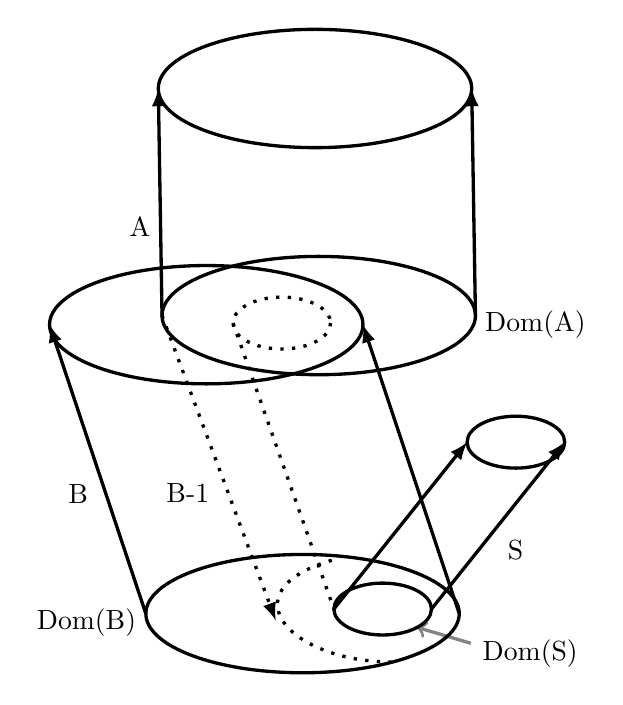
\begin{tikzpicture}
\pgftransformxscale{1.000000}
\pgftransformyscale{-1.000000}
\definecolor{dialinecolor}{rgb}{0.000000, 0.000000, 0.000000}
\pgfsetstrokecolor{dialinecolor}
\definecolor{dialinecolor}{rgb}{1.000000, 1.000000, 1.000000}
\pgfsetfillcolor{dialinecolor}
% setfont left to latex
\definecolor{dialinecolor}{rgb}{0.000000, 0.000000, 0.000000}
\pgfsetstrokecolor{dialinecolor}
\node[anchor=east] at (7.660000\du,14.450000\du){B };
% setfont left to latex
\definecolor{dialinecolor}{rgb}{0.000000, 0.000000, 0.000000}
\pgfsetstrokecolor{dialinecolor}
\node[anchor=east] at (9.165000\du,8.015000\du){A };
% setfont left to latex
\definecolor{dialinecolor}{rgb}{0.000000, 0.000000, 0.000000}
\pgfsetstrokecolor{dialinecolor}
\node[anchor=east] at (10.580000\du,14.422500\du){B-1 };
% setfont left to latex
\definecolor{dialinecolor}{rgb}{0.000000, 0.000000, 0.000000}
\pgfsetstrokecolor{dialinecolor}
\node[anchor=east] at (8.820000\du,17.557500\du){Dom(B) };
% setfont left to latex
\definecolor{dialinecolor}{rgb}{0.000000, 0.000000, 0.000000}
\pgfsetstrokecolor{dialinecolor}
\node[anchor=west] at (16.760000\du,10.377500\du){ Dom(A)};
% setfont left to latex
\definecolor{dialinecolor}{rgb}{0.000000, 0.000000, 0.000000}
\pgfsetstrokecolor{dialinecolor}
\node[anchor=west] at (17.305000\du,15.810000\du){ S};
% setfont left to latex
\definecolor{dialinecolor}{rgb}{0.000000, 0.000000, 0.000000}
\pgfsetstrokecolor{dialinecolor}
\node[anchor=west] at (16.700000\du,18.295000\du){ Dom(S)};
\pgfsetlinewidth{0.080000\du}
\pgfsetdash{}{0pt}
\pgfsetdash{}{0pt}
\pgfsetbuttcap
{
\definecolor{dialinecolor}{rgb}{0.517647, 0.517647, 0.517647}
\pgfsetfillcolor{dialinecolor}
% was here!!!
\pgfsetarrowsstart{to}
\definecolor{dialinecolor}{rgb}{0.517647, 0.517647, 0.517647}
\pgfsetstrokecolor{dialinecolor}
\draw (15.355850\du,17.666942\du)--(16.650000\du,18.050000\du);
}
\pgfsetlinewidth{0.080000\du}
\pgfsetdash{}{0pt}
\pgfsetdash{}{0pt}
\definecolor{dialinecolor}{rgb}{0.000000, 0.000000, 0.000000}
\pgfsetstrokecolor{dialinecolor}
\pgfpathellipse{\pgfpoint{10.275000\du}{10.375000\du}}{\pgfpoint{3.775000\du}{0\du}}{\pgfpoint{0\du}{1.425000\du}}
\pgfusepath{stroke}
\pgfsetlinewidth{0.080000\du}
\pgfsetdash{}{0pt}
\pgfsetdash{}{0pt}
\definecolor{dialinecolor}{rgb}{0.000000, 0.000000, 0.000000}
\pgfsetstrokecolor{dialinecolor}
\pgfpathellipse{\pgfpoint{12.985000\du}{10.155000\du}}{\pgfpoint{3.775000\du}{0\du}}{\pgfpoint{0\du}{1.425000\du}}
\pgfusepath{stroke}
\pgfsetlinewidth{0.080000\du}
\pgfsetdash{}{0pt}
\pgfsetdash{}{0pt}
\definecolor{dialinecolor}{rgb}{0.000000, 0.000000, 0.000000}
\pgfsetstrokecolor{dialinecolor}
\pgfpathellipse{\pgfpoint{12.895000\du}{4.685000\du}}{\pgfpoint{3.775000\du}{0\du}}{\pgfpoint{0\du}{1.425000\du}}
\pgfusepath{stroke}
\pgfsetlinewidth{0.080000\du}
\pgfsetdash{}{0pt}
\pgfsetdash{}{0pt}
\pgfsetbuttcap
{
\definecolor{dialinecolor}{rgb}{0.000000, 0.000000, 0.000000}
\pgfsetfillcolor{dialinecolor}
% was here!!!
\pgfsetarrowsend{latex}
\definecolor{dialinecolor}{rgb}{0.000000, 0.000000, 0.000000}
\pgfsetstrokecolor{dialinecolor}
\draw (9.210000\du,10.155000\du)--(9.120000\du,4.685000\du);
}
\pgfsetlinewidth{0.080000\du}
\pgfsetdash{}{0pt}
\pgfsetdash{}{0pt}
\pgfsetbuttcap
{
\definecolor{dialinecolor}{rgb}{0.000000, 0.000000, 0.000000}
\pgfsetfillcolor{dialinecolor}
% was here!!!
\pgfsetarrowsend{latex}
\definecolor{dialinecolor}{rgb}{0.000000, 0.000000, 0.000000}
\pgfsetstrokecolor{dialinecolor}
\draw (16.760000\du,10.155000\du)--(16.670000\du,4.685000\du);
}
\pgfsetlinewidth{0.080000\du}
\pgfsetdash{}{0pt}
\pgfsetdash{}{0pt}
\definecolor{dialinecolor}{rgb}{0.000000, 0.000000, 0.000000}
\pgfsetstrokecolor{dialinecolor}
\pgfpathellipse{\pgfpoint{12.595000\du}{17.335000\du}}{\pgfpoint{3.775000\du}{0\du}}{\pgfpoint{0\du}{1.425000\du}}
\pgfusepath{stroke}
\pgfsetlinewidth{0.080000\du}
\pgfsetdash{}{0pt}
\pgfsetdash{}{0pt}
\pgfsetbuttcap
{
\definecolor{dialinecolor}{rgb}{0.000000, 0.000000, 0.000000}
\pgfsetfillcolor{dialinecolor}
% was here!!!
\pgfsetarrowsend{latex}
\definecolor{dialinecolor}{rgb}{0.000000, 0.000000, 0.000000}
\pgfsetstrokecolor{dialinecolor}
\draw (16.370000\du,17.335000\du)--(14.050000\du,10.375000\du);
}
\pgfsetlinewidth{0.080000\du}
\pgfsetdash{}{0pt}
\pgfsetdash{}{0pt}
\pgfsetbuttcap
{
\definecolor{dialinecolor}{rgb}{0.000000, 0.000000, 0.000000}
\pgfsetfillcolor{dialinecolor}
% was here!!!
\pgfsetarrowsend{latex}
\definecolor{dialinecolor}{rgb}{0.000000, 0.000000, 0.000000}
\pgfsetstrokecolor{dialinecolor}
\draw (8.820000\du,17.335000\du)--(6.500000\du,10.375000\du);
}
\pgfsetlinewidth{0.080000\du}
\pgfsetdash{{\pgflinewidth}{0.200000\du}}{0cm}
\pgfsetdash{{\pgflinewidth}{0.200000\du}}{0cm}
\pgfsetmiterjoin
\pgfsetbuttcap
{
\definecolor{dialinecolor}{rgb}{0.000000, 0.000000, 0.000000}
\pgfsetfillcolor{dialinecolor}
% was here!!!
\definecolor{dialinecolor}{rgb}{0.000000, 0.000000, 0.000000}
\pgfsetstrokecolor{dialinecolor}
\pgfpathmoveto{\pgfpoint{13.300000\du}{16.050000\du}}
\pgfpathcurveto{\pgfpoint{10.750000\du}{16.800000\du}}{\pgfpoint{12.300000\du}{18.500000\du}}{\pgfpoint{14.750000\du}{18.500000\du}}
\pgfusepath{stroke}
}
\pgfsetlinewidth{0.080000\du}
\pgfsetdash{{\pgflinewidth}{0.200000\du}}{0cm}
\pgfsetdash{{\pgflinewidth}{0.200000\du}}{0cm}
\pgfsetbuttcap
{
\definecolor{dialinecolor}{rgb}{0.000000, 0.000000, 0.000000}
\pgfsetfillcolor{dialinecolor}
% was here!!!
\pgfsetarrowsend{latex}
\definecolor{dialinecolor}{rgb}{0.000000, 0.000000, 0.000000}
\pgfsetstrokecolor{dialinecolor}
\draw (9.210000\du,10.155000\du)--(11.950000\du,17.500000\du);
}
\pgfsetlinewidth{0.080000\du}
\pgfsetdash{}{0pt}
\pgfsetdash{}{0pt}
\definecolor{dialinecolor}{rgb}{0.000000, 0.000000, 0.000000}
\pgfsetstrokecolor{dialinecolor}
\pgfpathellipse{\pgfpoint{14.525000\du}{17.225000\du}}{\pgfpoint{1.175000\du}{0\du}}{\pgfpoint{0\du}{0.625000\du}}
\pgfusepath{stroke}
\pgfsetlinewidth{0.080000\du}
\pgfsetdash{}{0pt}
\pgfsetdash{}{0pt}
\definecolor{dialinecolor}{rgb}{0.000000, 0.000000, 0.000000}
\pgfsetstrokecolor{dialinecolor}
\pgfpathellipse{\pgfpoint{17.735000\du}{13.205000\du}}{\pgfpoint{1.175000\du}{0\du}}{\pgfpoint{0\du}{0.625000\du}}
\pgfusepath{stroke}
\pgfsetlinewidth{0.080000\du}
\pgfsetdash{}{0pt}
\pgfsetdash{}{0pt}
\pgfsetbuttcap
{
\definecolor{dialinecolor}{rgb}{0.000000, 0.000000, 0.000000}
\pgfsetfillcolor{dialinecolor}
% was here!!!
\pgfsetarrowsend{latex}
\definecolor{dialinecolor}{rgb}{0.000000, 0.000000, 0.000000}
\pgfsetstrokecolor{dialinecolor}
\draw (13.350000\du,17.225000\du)--(16.560000\du,13.205000\du);
}
\pgfsetlinewidth{0.080000\du}
\pgfsetdash{}{0pt}
\pgfsetdash{}{0pt}
\pgfsetbuttcap
{
\definecolor{dialinecolor}{rgb}{0.000000, 0.000000, 0.000000}
\pgfsetfillcolor{dialinecolor}
% was here!!!
\pgfsetarrowsend{latex}
\definecolor{dialinecolor}{rgb}{0.000000, 0.000000, 0.000000}
\pgfsetstrokecolor{dialinecolor}
\draw (15.700000\du,17.225000\du)--(18.910000\du,13.205000\du);
}
\pgfsetlinewidth{0.080000\du}
\pgfsetdash{{\pgflinewidth}{0.200000\du}}{0cm}
\pgfsetdash{{\pgflinewidth}{0.200000\du}}{0cm}
\definecolor{dialinecolor}{rgb}{0.000000, 0.000000, 0.000000}
\pgfsetstrokecolor{dialinecolor}
\pgfpathellipse{\pgfpoint{12.095000\du}{10.335000\du}}{\pgfpoint{1.175000\du}{0\du}}{\pgfpoint{0\du}{0.625000\du}}
\pgfusepath{stroke}
\pgfsetlinewidth{0.080000\du}
\pgfsetdash{{\pgflinewidth}{0.200000\du}}{0cm}
\pgfsetdash{{\pgflinewidth}{0.200000\du}}{0cm}
\pgfsetbuttcap
{
\definecolor{dialinecolor}{rgb}{0.000000, 0.000000, 0.000000}
\pgfsetfillcolor{dialinecolor}
% was here!!!
\definecolor{dialinecolor}{rgb}{0.000000, 0.000000, 0.000000}
\pgfsetstrokecolor{dialinecolor}
\draw (10.920000\du,10.335000\du)--(13.350000\du,17.225000\du);
}
\end{tikzpicture}
 % TODO arrows too small

We see that the set of filesystems the sequences in $\seqset{A}$ do not break intersect with the range of $B$.
As $B$ is a bijection between its domain and range, we can use $B^{-1}$ to map this intersection back
onto the domain of $B$.
As $\worksc{B\cc \seqset{A}}{\seqset{S}}$ the domain of $\seqset{S}$ must be a subset of this
projected intersection.
If so, then we can use $B$ to map the domain of $\seqset{S}$, which yields the domain of $B^{-1}\cc \seqset{S}$.
As it is also a part of the domain of $A$, we get $\worksc{\seqset{A}}{B^{-1}\cc \seqset{S}}$.

The second part of the lemma can be proven in a similar way.
\end{proof}


\begin{mylem}\label{indep_prefix_combine}
The combination of sequences with a common head and independent tails 
continues to work under the same conditions:
\[ \worksc{A\cc B}{\seqset{S}} \wedge \worksc{A\cc C}{\seqset{S}} \wedge B\indep C \Rightarrow \worksc{A\cc B\cc C}{\seqset{S}} \]
\end{mylem}
\begin{proof}
Based on \cref{r_invmove} we know
$\worksc{B}{A^{-1}\cc \seqset{S}}$ and $\worksc{C}{A^{-1}\cc \seqset{S}}$,
and from \cref{combine_independent_sequences} we know
$\worksc{B\cc C}{B,C}$.
Combining these using \cref{workschained}
we get
$\worksc{B\cc C}{A^{-1}\cc \seqset{S}}$. 
Finally, applying the second line of \cref{r_invmove} yields
$\worksc{(A^{-1})^{-1}\cc B\cc C}{\seqset{S}}$, which proves our lemma 
as $\forall\FS: (A^{-1})^{-1}\FS\typeeq A\FS$ (\cref{negneg_is_typeeq}).
\end{proof}
